\chapter{Implementation and Testing}

\section{FileSync.py application}
Application goal explained in~\autoref{file-sync}
Appendix code~\autoref{apx:file-sync-code}

FileSync is a python application that will synchronize all files in a specified path, with all participants within the synchronization room.

\section{Application.py}
Application flow explained in~\autoref{sensor-application}

\subsection{Packet Design}
Initialization packets are limited to the structure in~\autoref{fig:init_interest-data}
Sensor packets are limited to the structure in~\autoref{fig:sensor_interest-data}
\begin{description}
	\item[Init Interest]
	\item[Init Data]
	\item[Sensor Interest]
	KeyLocator can be of type Name. 
	As described in the \gls{NDN} Packet Format, generally this field can be used to specify where to download the certificate used to sign the Interest.
	However, in our trust model we use this field to publish the requesters Name, i.e. the requesters public key. 
	\item[Sensor Data]
\end{description}

\begin{figure}[ht]
  \centering
  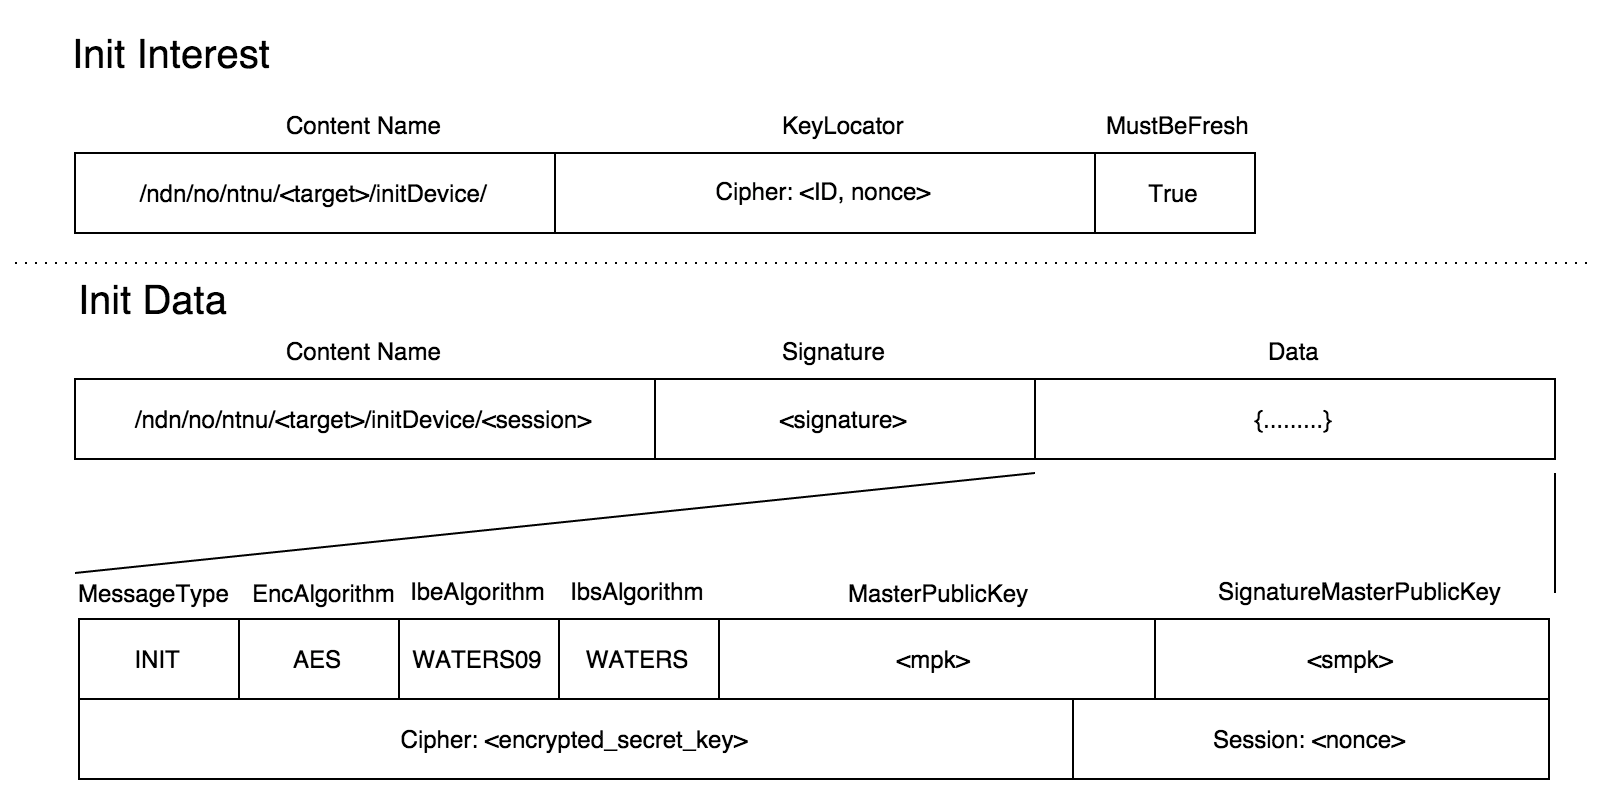
\includegraphics[width=1\textwidth]{init_interest-data.png}
  \caption{Initialization Interest and Data}
  \label{fig:init_interest-data}
\end{figure}

\begin{figure}[ht]
  \centering
  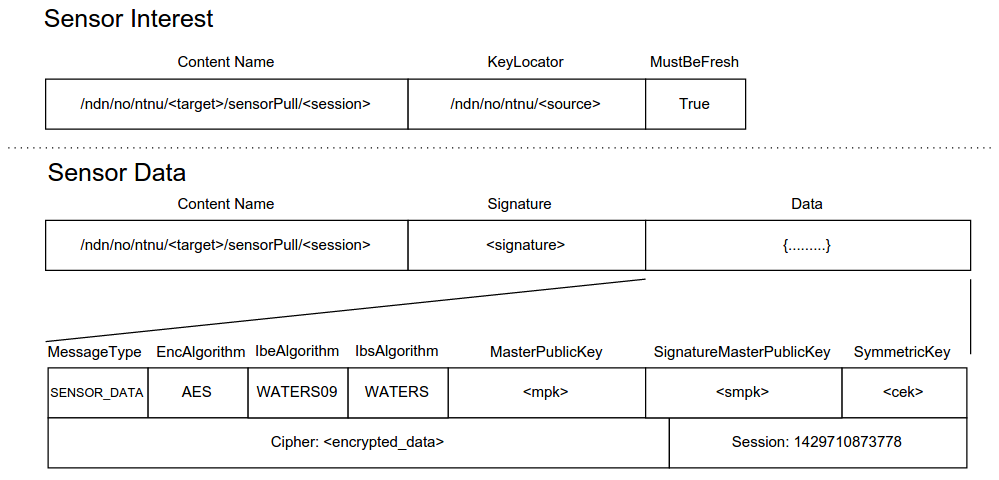
\includegraphics[width=1\textwidth]{sensor_interest-data.png}
  \caption{Sensor Interest and Data}
  \label{fig:sensor_interest-data}
\end{figure}